\subsection{Class diagram}
  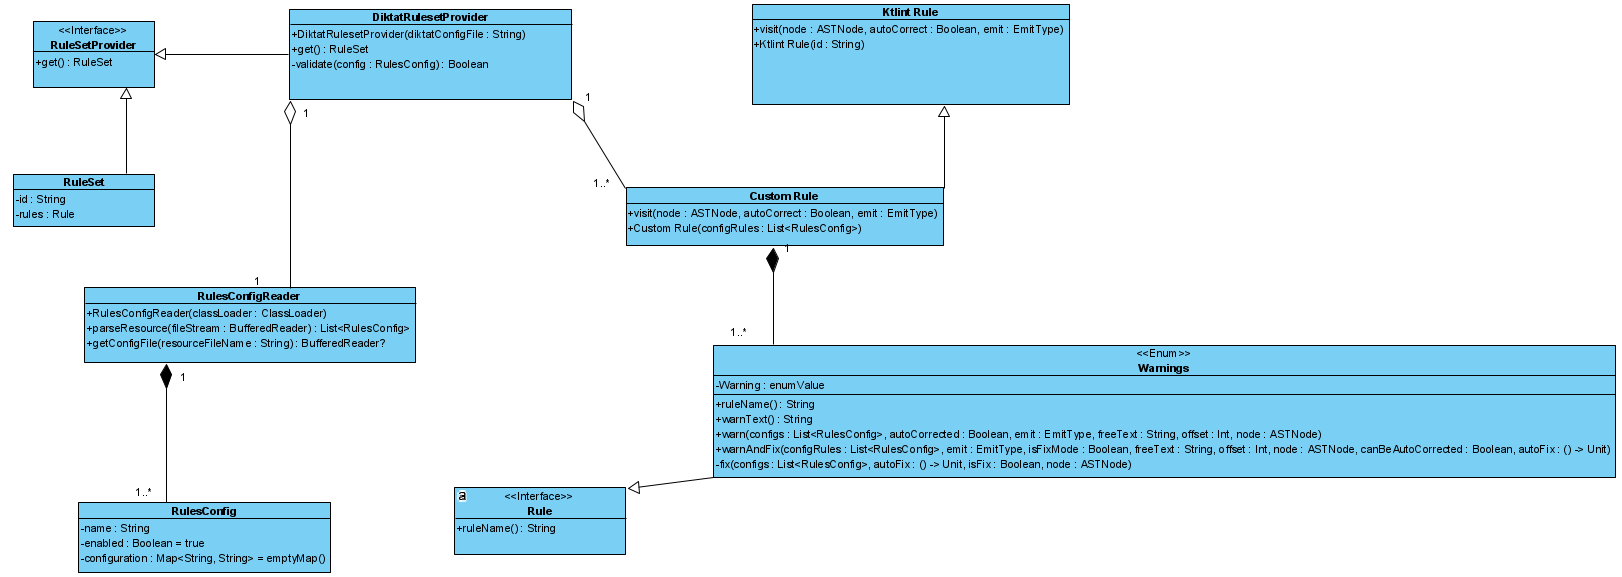
\includegraphics[scale=0.5]{pictures/class.PNG}

\subsection{Data Flow diagram}
  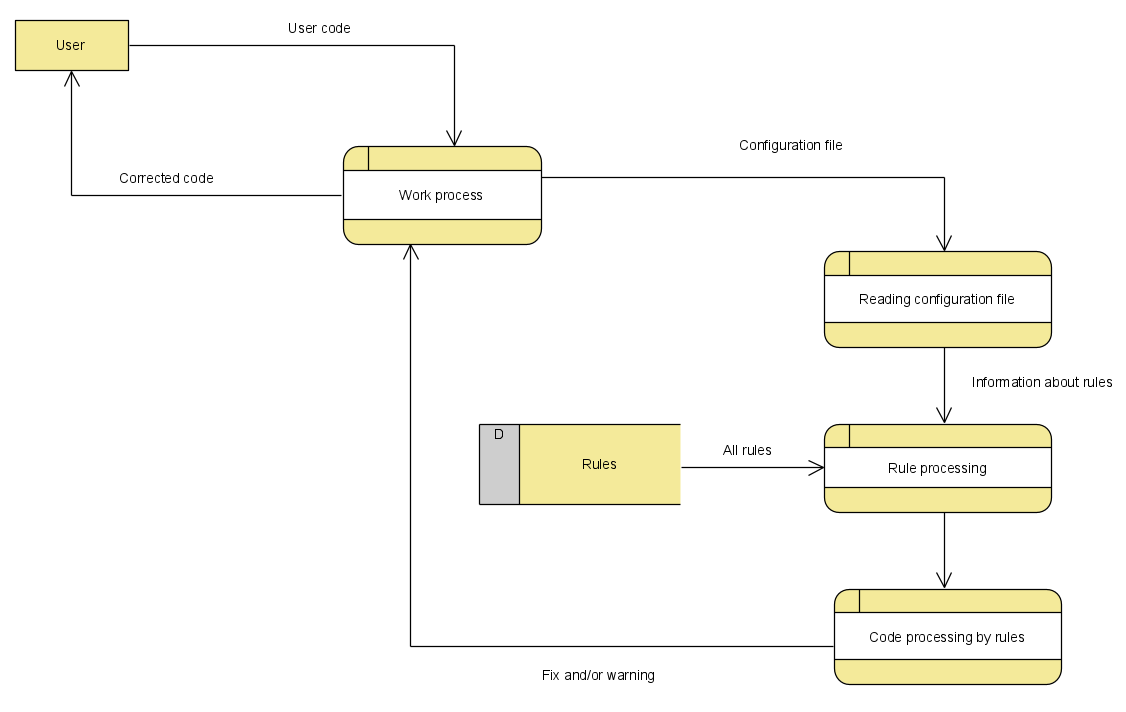
\includegraphics[scale=0.6]{pictures/data_flow.PNG}

\subsection{Sequence diagram}
  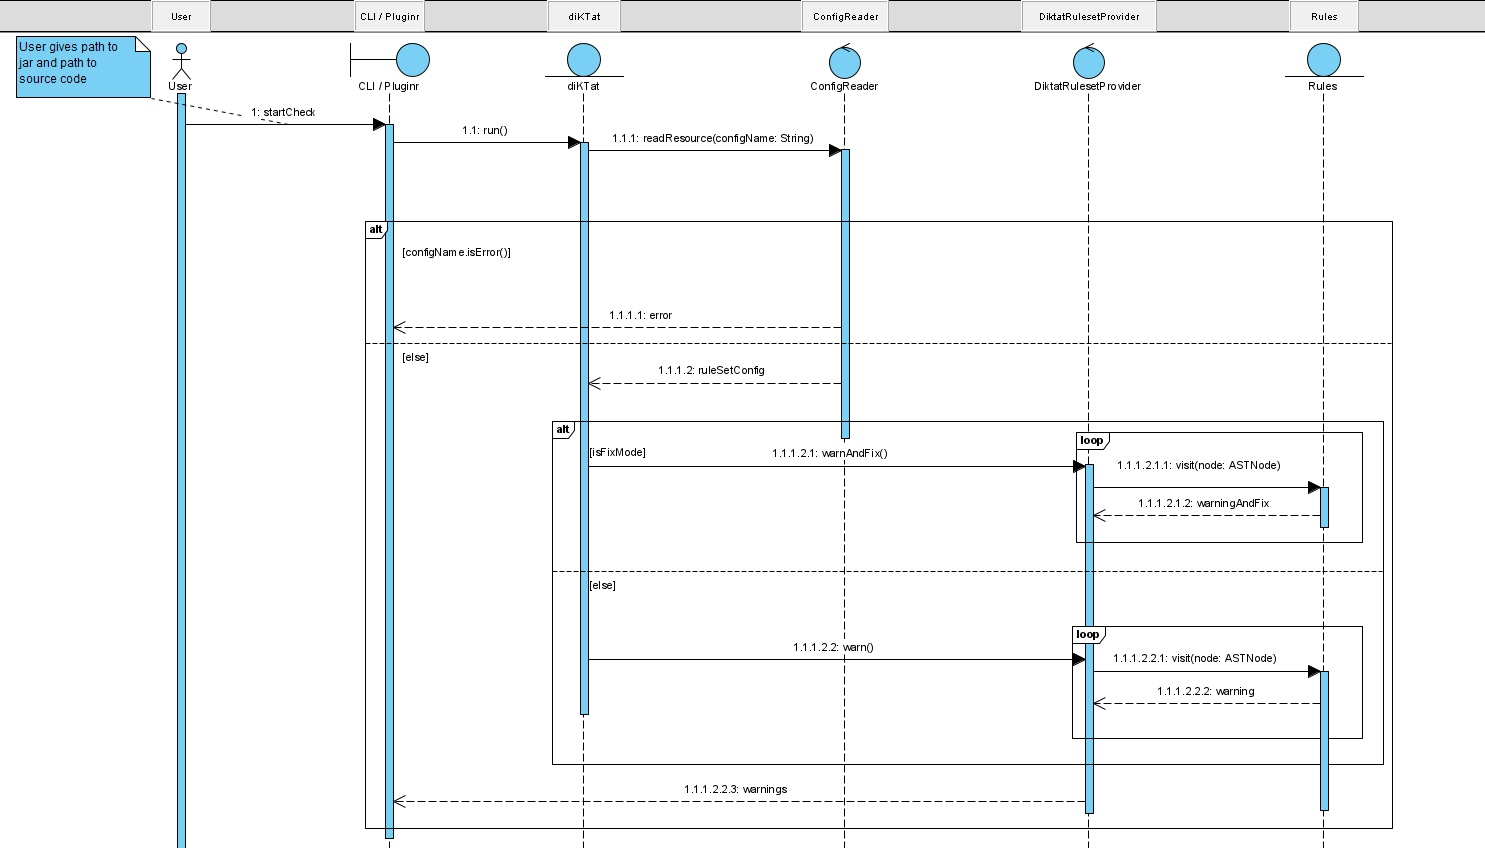
\includegraphics[scale=0.33]{pictures/sequence.jpg}

\section*{guide}

\lstMakeShortInline[basicstyle=\ttfamily\bfseries]`

\section*{\textbf{Preface}}

\subsection*{\textbf{Purpose of this document}}



For code to be considered "good", it must entail the following characteristics:

1.	Simplicity

2.	Maintainability

3.	Reliability

4.	Testability

5.	Efficiency

6.	Portability

7.	Reusability



Programming is a profession that involves creativity.

Software developers can reference this specification, which will enhance their ability to write consistent, easy-to-read, and high-quality code.

This will ultimately improve product competitiveness and software development efficiency.



\subsection*{\textbf{General principles}}



As a very modern and advanced programming language (completely like other languages), Kotlin complies with the following general principles:

1.	Clarity: Clarity is a necessary feature of programs that are easy to maintain and refactor.

2.	Simplicity: Simple code is easy to understand and implement.

3.	Consistency: Unification is particularly important when the same team works on the same project, utilizing similar styles. It enables code to be easily modified, reviewed, and understood by the team members.



In addition, we need to consider the following factors when programming on Kotlin:



1. Write clean and simple Kotlin code



    Kotlin combines two of the main programming paradigms: functional and object-oriented.

    Both of these paradigms are trusted, well-known software engineering practices.

    As a young programming language, Kotlin builds on well-established languages such as Java, C++, C\#, and Scala.

    This is why Kotlin introduces many features that help you write cleaner, more readable code, while also reducing the number of complex code structures. For example: type and null safety, extension functions, infix syntax, immutability, val/var differentiation, expression-oriented features, when statements, much easier work with collections, type auto conversion, and other syntactic sugar.



2. Follow Kotlin idioms



    The author of Kotlin, Andrey Breslav, mentioned that it is both pragmatic and practical, but not academic.

    Its pragmatic features enable ideas to easily be transformed into real working software. This programming language is closer to natural languages than its predecessors, and it implements the following design principles: readability, reusability, interoperability, security, and tool-friendliness (https://blog.jetbrains.com/kotlin/2018/10/kotlinconf-2018-announcements/).



3. Use Kotlin efficiently



    Some Kotlin features help you write higher-performance code: including rich coroutine library, sequences, inline functions/classes, arrays of basic types, tailRec, and CallsInPlace of contract.



\subsection*{\textbf{Terminology}}



\textbf{Rules}: conventions that should be followed when programming.



\textbf{Recommendations}: conventions that should be considered when programming.



\textbf{Explanation}: necessary explanations of rules and recommendations.



\textbf{Valid Example}: examples (recommended) of rules and recommendations.



\textbf{Invalid Example}: examples (not recommended) of rules and recommendations.



Unless otherwise stated, this specification applies to versions 1.3 and later of Kotlin.



\subsection*{\textbf{Exceptions}}



Even though exceptions may exist, it is important to understand why rules and recommendations are needed.

Depending on your project situation or personal habits, you can break some of the rules. However, remember that one exception leads to many and can completely destroy the consistency of code. As such, there should be very few exceptions.

When modifying open-source code or third-party code, you can choose to implement the style used by the code (as opposed to using the existing specifications) to maintain consistency.

Software that is directly based on the interface of the Android native operating system, such as the Android Framework, remains consistent with the Android style.

\section*{\textbf{1. Naming}}

In programming, it is difficult to meaningfully and appropriately name variables, functions, classes, etc. Good names clearly express the main ideas and functionality of your code, as well as avoid misinterpretation, unnecessary coding and decoding, magic numbers, and inappropriate abbreviations.



\subsubsection*{\textbf{Rule 1.0.1}}
\leavevmode\newline

The source file encoding format (including comments) must be UTF-8 only. The ASCII horizontal space character (0x20, that is, space) is the only permitted whitespace character. Tabs should not be used for indentation.



\subsection*{\textbf{1.1 Identifiers naming}}

\subsubsection*{\textbf{Rule 1.1.1}}
\leavevmode\newline

1.	All identifiers should use only ASCII letters or digits, and the names should match regular expressions `\w{2,64}`.

Explanation: Each valid identifier name should match the regular expression `\w{2,64}`.

`{2,64}` means that the name length is 2 to 64 characters, and the length of the variable name should be proportional to its life range, functionality, and responsibility.

Name lengths of less than 31 characters are generally recommended, but this depends on the project. Otherwise, class declaration with generics or inheritance from a super class can cause line breaking for example. No special prefix or suffix should be used in the names. The following examples are inappropriate: name\_, mName, s\_name, and kName.



2.	For files, choose names that describe their content. Use camel case (PascalCase) and `.kt` extension.



3.	Typical examples of naming:



\begin{center}

\begin{tabular}{ |p{5,0cm}|p{5,0cm}|p{5,0cm}| }

\hline

Meaning&Correct&Incorrect\\

\hline

 "XML Http Request" & XmlHttpRequest & XMLHTTPRequest \\

 "new customer ID" & newCustomerId & newCustomerID \\

 "inner stopwatch" & innerStopwatch & innerStopWatch \\

 "supports IPv6 on iOS" & supportsIpv6OnIos & supportsIPv6OnIOS \\

 "YouTube importer" & YouTubeImporter & YoutubeImporter \\

\hline

\end{tabular}

\end{center}

4.	The usage of (``) and free naming for functions and identifiers are prohibited. For example, the following code is not recommended:



\begin{lstlisting}[language=Kotlin]
val `my dummy name-with-minus` = "value" 
\end{lstlisting}


The only exception is function names in `Unit tests`.



5.	Backticks (``) should not be used for identifiers, except the names of test methods (marked with @Test annotation):

\begin{lstlisting}[language=Kotlin]
 @Test fun `my test`() { /*...*/ }
\end{lstlisting}
6.  The following table contains some characters that cause confusion. Be careful when using them as identifiers, or use other names instead.



\begin{center}

\begin{tabular}{ |p{5,0cm}|p{5,0cm}|p{5,0cm}| }

\hline

Expected&Confusing name&Suggested name\\

\hline

 0 (zero)      & O, D                     & obj, dgt         \\

 1 (one)       & I, l                     & it, ln, line     \\

 2 (two)       & Z                        & n1, n2           \\

 5 (five)      & S                        & xs, str          \\

 6 (six)       & e                        & ex, elm          \\

 8 (eight)     & B                        & bt, nxt          \\

 n,h           & h,n                      & nr, head, height \\

 rn, m         & m,rn                     & mbr, item        \\

\hline

\end{tabular}

\end{center}

\textbf{Exceptions}

- The i,j,k variables used in loops are part of the industry standard. One symbol can be used for for such variables.

- The `e` variable can be used to catch exceptions in catch block: `catch (e: Exception) {}`

- The Java community generally does not recommend the use of prefixes; however, when developing Android code, you can use the s and m prefixes for static and non-public non-static fields, respectively.

Note that prefixing can also negatively affect the style, as well as the auto generation of getters and setters.



\begin{center}

\begin{tabular}{ |p{7,5cm}|p{7,5cm}| }

\hline

Type&Naming style\\

\hline

 Interfaces, classes, annotations, enumerated types, and object type names & Camel case starting with a capital letter. Test classes have a Test suffix. The filename is 'TopClassName'.kt.  \\

 Class fields, local variables, methods, and method parameters & Camel case starting with a small letter. Test methods may be underlined with '\_'., the only exception is [backing properties] \\

 Static constants and enumerated values & Only uppercase underlined with '\_' \\

 Generic type variable & Single capital letter, which can be followed by a number, for example: `E, T, U, X, T2` \\

 Exceptions & Same as class names, but with a suffix Exception, for example: `AccessException` and `NullPointerException`\\

\hline

\end{tabular}

\end{center}

\subsection*{\textbf{1.2 Packages names}}

\subsubsection*{\textbf{Rule 1.2.1}}
\leavevmode\newline

Package names are all written in lowercase, and consecutive words are simply concatenated together (no underscores). Package names should contain both the product and module names, as well as the department or team name to prevent conflicts with other teams.  Numbers are not permitted. For example: `org.apache.commons.lang3`, `xxx.yyy.v2`.



\textbf{Exceptions:} 



- In certain cases, such as open-source projects or commercial cooperation, package names should not start with `your.company.domain`.- In some cases, if the package name starts with a number or other characters, but these characters cannot be used at the beginning of the Java/Kotlin package name, or the package name contains reserved Java keywords, underscores are allowed.

- Underscores are sometimes permitted if the package name starts with a number or other character, which cannot be used at the beginning of the Java/Kotlin package name; or the package name contains reserved Java keywords. For example: org.example.hyphenated\_name, int\_.example, com.example.\_123name   

For example: `org.example.hyphenated\_name`,` int\_.example`, `com.example.\_123name`



\textbf{Valid example}: 

\begin{lstlisting}[language=Kotlin]
package your.company.domain.mobilecontrol.views
\end{lstlisting}


\subsection*{\textbf{1.3 Classes}}

\subsubsection*{\textbf{Rule 1.3.1}}
\leavevmode\newline



1.	The class name is usually a noun or a noun phrase using the camel case nomenclature, such as UpperCamelCase. For example: `Character` or `ImmutableList`.

The name of an interface can also be a noun or noun phrase (such as `List`), or an adjective or adjective phrase (such as `Readable`).

Note that verbs should not be used to name classes; however, nouns (such as `Customer`, `WikiPage`, and `Account`) can be used. Try to avoid vague words like Manager and Process.



2.	Test classes start with the name of the class they are testing and end with Test. For example: HashTest or HashIntegrationTest



\textbf{Invalid example}: 

\begin{lstlisting}[language=Kotlin]
class marcoPolo {} 
class XMLService {} 
interface TAPromotion {}
class info {}
\end{lstlisting}


\textbf{Valid example}: 

\begin{lstlisting}[language=Kotlin]
class MarcoPolo {}
class XmlService {}
interface TaPromotion {}
class Order {}
\end{lstlisting}


\subsection*{\textbf{1.4 Functions}}

\subsubsection*{\textbf{Rule 1.4.1}}
\leavevmode\newline



1.	Function names are usually verbs or verb phrases, and use the camel case nomenclature (`lowerCamelCase`).

For example: `sendMessage`, `stopProcess`, or `calculateValue`.

The format is as follows:



a) To get, modify, or calculate a certain value: get + non-boolean field(). However, note that getters are automatically generated by the Kotlin compiler for some classes, and the special get syntax is preferred for fields: kotlin private val field: String get() { }.

\begin{lstlisting}[language=Kotlin]
private val field: String
get() {
}
\end{lstlisting}
Additionally, calling property access syntax is preferred to calling getter directly. (In this case, the Kotlin compiler will automatically call the corresponding getter).



b) `is` + boolean variable name()



c) `set` + field/attribute name(). However, note that the syntax and code generation for Kotlin are completely the same as those described for the getters in point a.



d) `has` + Noun / adjective ()



e) verb()

The verb is mainly used on the object of the action itself, such as `document.print ()`



f) verb + noun() 



g) The Callback function allows for names that use the preposition + verb format, such as: `onCreate()`, `onDestroy()`, `toString()`.



\textbf{Invalid example}: 



\begin{lstlisting}[language=Kotlin]
fun type(): String
fun Finished(): Boolean
fun visible(boolean)
fun DRAW()
fun KeyListener(Listener)
\end{lstlisting}


\textbf{Valid example}: 



\begin{lstlisting}[language=Kotlin]
fun getType(): String
fun isFinished(): Boolean
fun setVisible(boolean)
fun draw()
fun addKeyListener(Listener)
\end{lstlisting}


2.	An underscore can be included in the JUnit test function name, and should be a logical component used to separate names. Each logical part is written in lowerCamelCase. For example: a typical pattern \_, such as pop\_emptyStack



\subsection*{\textbf{1.5 Constants}}

\subsubsection*{\textbf{Rule 1.5.1 Constant names should be in UPPER case}}
\leavevmode\newline



1.	Constants are attributes created with the const keyword, or top-level/`val` local variables of an object that holds immutable data. In most cases, constants can be identified as a `const val` property from the `object`/`companion object`/file top level. These variables contain a fixed constant value that typically should never be changed by programmers. This includes basic types, strings, immutable types, and immutable collections of immutable types. If an object state can be changed, the value is not a constant.



2. Constant names should contain only uppercase letters separated by underscores. They should have a val or const val modifier to explicitly make them final. In most cases, if you need to specify a constant value, then you need to create it with the "const val" modifier. Note that not all `val` variables are constants.



3. Objects that have immutable content, such as `Logger` and `Lock`, can be in uppercase as constants or have camel case as regular variables.



4. Use meaningful constants instead of `magic numbers`. SQL or logging strings should not be treated as magic numbers, nor should they be defined as string constants.

Magic constants like `NUM\_FIVE = 5` or `NUM\_5 = 5` should not be treated as constants. This is because mistakes will easily be made if they are changed to `NUM\_5 = 50` or 55.

Typically, these constants represent business logic values like measures, capacity, scope, location, tax rate, promotional discounts, and power base multiples in algorithms. 

Magic numbers can be avoided through the following methods:

- Using library functions and APIs. For example, instead of checking that `size == 0`, use `isEmpty()` function. To work with `time`, use built-ins from `java.time API`.

- Enumerations can be used to name patterns. Refer to [Recommended usage scenario for enumeration in 3.9]



\textbf{Invalid example}: 



\begin{lstlisting}[language=Kotlin]
var int MAXUSERNUM = 200;
val String sL = "Launcher";
\end{lstlisting}


\textbf{Valid example}:



\begin{lstlisting}[language=Kotlin]
const val int MAX_USER_NUM = 200;
const val String APPLICATION_NAME = "Launcher";
\end{lstlisting}


\subsection*{\textbf{1.6 Non-constant fields}}

\subsubsection*{\textbf{Rule 1.6.1}}
\leavevmode\newline



A local variable cannot be treated as a constant even if it is final and immutable. Therefore, it should not use the preceding rules. The name of variables with a type from collections (sets, lists, etc.) should contain plural nouns.

For example: `var namesList: List<String>`



Names of non-constant variables should use lower camel case. The name of the final immutable field used to store the singleton object can use the same notation with camel case.



\textbf{Invalid example}: 

\begin{lstlisting}[language=Kotlin]
customername: String
user: List<String> = listof()
\end{lstlisting}


\textbf{Valid example}: 

\begin{lstlisting}[language=Kotlin]
var customerName: String
val users: List<String> = listOf();
val mutableCollection: MutableSet<String> = HashSet()
\end{lstlisting}


\subsubsection*{\textbf{Recommendation 1.6.2}}
\leavevmode\newline



\textit{Note}: When using a logical operator and name with negative meaning, the code may be difficult to understand, which is referred to as the "double negative".

For instance, it is not easy to understand the meaning of !isNotError.

The JavaBeans specification automatically generates isXxx() getters for attributes of Boolean classes.

However, methods that return Boolean type do not all have this notation.

For Boolean local variables or methods, it is highly recommended that you add non-meaningful prefixes, including is (which is commonly used by JavaBeans), or has, can, should, must. Modern integrated development environments (IDEs) such as Intellij are already capable of doing this for you when you generate getters in Java. For Kotlin, this process is even easier as everything is on the byte-code level under the hood.



\textbf{Invalid example}: 

\begin{lstlisting}[language=Kotlin]
val isNoError: Boolean
val isNotFound: Boolean
fun empty()
fun next();
\end{lstlisting}


\textbf{Valid example}:

\begin{lstlisting}[language=Kotlin]
val isError: Boolean
val isFound: Boolean
val hasLicense: Boolean
val canEvaluate: Boolean
val shouldAbort: Boolean
fun isEmpty()
fun hasNext()
\end{lstlisting}
\section*{\textbf{2. Comments}}



The best practice involves beginning your code with a short summary, which can be one sentence.

You should balance between writing no comments at all and obvious comments for each line of code.

Comments should be accurately and clearly expressed, without repeating the name of the class, interface, or method.

Comments are not a solution to bad code. Instead, you should fix the code as soon as you notice an issue, or plan to fix it (with a TODO comment including a Jira number).

Comments should accurately reflect the design ideas and logic of the code, and then describe the code's business logic.

As a result, other programmers will be able to save time when trying to understand the code.

Imagine that you are writing the comments to help your future self understand the original ideas behind the code. 



\subsection*{\textbf{2.1 General form of Kdoc}}

 

KDoc is a combination of JavaDoc's block tags syntax (extended to support specific constructions of Kotlin) and Markdown's inline markup.

The basic format of KDoc is shown in the following example:



\begin{lstlisting}[language=Kotlin]
 /**
 * There are multiple lines of KDoc text,
 * Other ...
 */
fun method(arg: String) {
    // …
}
\end{lstlisting}


It is also shown in the following single-line form:



\begin{lstlisting}[language=Kotlin]
 /** Short form of KDoc. */
\end{lstlisting}
When the entire KDoc block can be stored in one line (and there is no KDoc mark @XXX), a single-line form can be used. For detailed instructions on how to use KDoc, refer to [Official Document](https://docs.oracle.com/en/Kotlin/Kotlinse/11/tools/KDoc.html).



\subsubsection*{\textbf{Rule 2.1.1}}
\leavevmode\newline



At a minimum, KDoc should be used for every public, protected, or internal decorated class, interface, enumeration, method, and member field (property). Other code blocks can also have KDocs if needed.



Exceptions:



1. For setters/getters of properties obvious comments are optional.

 (Note that simple `get/set` methods are generated by Kotlin under the hood). For example, getFoo can also be `return foo`.

   

2. It is optional to add comments for simple one-line methods like:

\begin{lstlisting}[language=Kotlin]
val isEmpty: Boolean
    get() = this.size == 0
\end{lstlisting}


or



\begin{lstlisting}[language=Kotlin]
fun isEmptyList(list: List<String>) = list.size == 0
\end{lstlisting}


3. You can skip KDocs for a method's override if the method is almost like the super class method.



\subsubsection*{\textbf{Rule 2.1.2}}
\leavevmode\newline



\textbf{Valid examples}:



\begin{lstlisting}[language=Kotlin]
/** 
 * This is the short overview comment for the example interface.
 *     / * Add a blank line between the comment text and each KDoc tag underneath * /
 * @since 2019-01-01
 */
 protected abstract class Sample {
    /**
     * This is a long comment with whitespace that should be split in 
     * comments on multiple lines in case the line comment formatting is enabled.
     *     / * Add a blank line between the comment text and each KDoc tag underneath * /
     * @param fox A quick brown fox jumps over the lazy dog
     * @return battle between fox and dog 
     */
    protected abstract fun foo(Fox fox)
     /**
      * These possibilities include: Formatting of header comments
      *     / * Add a blank line between the comment text and each KDoc tag underneath * /
      * @return battle between fox and dog
      * @throws ProblemException if lazy dog wins
      */
    protected fun bar() throws ProblemException {
        // Some comments / * No need to add a blank line here * /   
        var aVar = ...

        // Some comments  / * Add a blank line before the comment * /   
        fun doSome()
    }
 }
\end{lstlisting}


\subsubsection*{\textbf{Rule 2.1.3}}
\leavevmode\newline



This is how Kdoc should look like and what it should contain:

- Functional and technical description, explaining the principles, intentions, contracts, API, etc.

- The function description and @tags (`implSpec`, `apiNote`, and `implNote`) require an empty line after them.

- `@implSpec`: A specification related to API implementation, and it should let the implementer decide whether to override it.

- `@apiNote`: Explain the API precautions, including whether to allow null and whether the method is thread safe, as well as the algorithm complexity, input and output range, exceptions, etc.

- `@implNote`: A note related to API implementation, which implementers should keep in mind.

- Then one empty line, followed by regular `@param`, `@return`, `@throws` and other comments.

- The conventional standard "block labels" are arranged in order: `@param`, `@return`, `@throws`.

- Empty descriptions in tag blocks are not permitted. It is better not to write Kdoc than to waste code line on empty space.

- There should be no empty lines between the method/class declaration and the end of Kdoc (`*/` symbols).

- (!) KDoc does not support the `@deprecated` tag. Instead, use the `@Deprecated` annotation.

 

If a tag block cannot be described in one line, you should indent the content of the new line by `4 spaces` from the `@` position to achieve alignment (`@` counts as one + three spaces).

 

\textbf{Exception:} When the descriptive text in a tag block is too long to wrap, the alignment can be indented with the descriptive text in the previous line. The descriptive text of multiple tags does not need to be aligned.

See [3.8 Horizontal space].



In Kotlin compared to Java you are able to put several classes inside one file so each class should have a Kdoc formatted comment (this is also stated in rule 2.1).

This comment should contain @since tag. The good style is to write the version of the application when functionality was released. It should be written after a `@since` tag.



\textbf{Examples:}



\begin{lstlisting}[language=Kotlin]
/**
 * Description of functionality
 *
 * @since 1.6
 */
\end{lstlisting}


Other KDoc tags (such as @param type parameters and @see.) can be added as follow:

\begin{lstlisting}[language=Kotlin]
/**
 * Description of functionality
 *
 * @apiNote: Important information about API
 *
 * @since 1.6
 */
\end{lstlisting}
\subsection*{\textbf{2.2 Comments to the file header}}

\subsubsection*{\textbf{Rule 2.2.1}}
\leavevmode\newline



Comments on the file header should be stored before the package name and imports. If you need to add more content to the comment, you can subsequently add it in the same format.



The following examples for Huawei describe the format of the \textbf{copyright license}: \

Chinese version: `版权所有 (c) 华为技术有限公司 2012-2020` \

English version: `Copyright (c) Huawei Technologies Co., Ltd. 2012-2020. All rights reserved.`



Regarding the \textbf{release notes}, see examples below:



- `2012-2020` can be modified according to your actual situation. `2012` and `2020` are the years the file was first created and last modified, respectively.

These two years can be the same (for example, `2020–2020`). When the file is substantially changed (for example, through feature extensions and major refactorings), the subsequent years must be updated.



- The \textbf{copyright statement} can use your company's subsidiaries. For example: \

Chinese version: `版权所有 (c) 海思半导体 2012-2020` \

English version: `Copyright (c) Hisilicon Technologies Co., Ltd. 2012-2020. All rights reserved.` 



- The copyright information should not be written in KDoc style or use single-line comments. It must start from the beginning of the file.

The following example is a copyright statement for Huawei, without other functional comments:



\begin{lstlisting}[language=Kotlin]
/*
 * Copyright (c) Huawei Technologies Co., Ltd. 2012-2020. All rights reserved.
 */
\end{lstlisting}


The following factors should be considered when writing the file header or comments for top-level classes:

- File header comments must start from the top of the file. If it is a top-level file comment, there should be a blank line after the last Kdoc `*/` symbol. If it is a comment for a top-level class, class declaration should start immediately without using a newline.

- Maintain a unified format. The specific format can be formulated by the project (for example, in opensource) and you need to follow it.

- A top-level file-Kdoc must include a copyright and functional description, especially if there is more than one top-level class.

- Do not include empty comment blocks. As described in the preceding example, if there is no content after the option `@apiNote`, the entire tag block should be deleted.

- The industry does not include historical information in comments. The corresponding history can be found in VCS (git, svn, etc.). As such, it is not recommended to include historical data in the comments of the Kotlin source code.





\subsection*{\textbf{2.3 Comments on the function header}}

\subsubsection*{\textbf{Rule 2.3.1}}
\leavevmode\newline

Comments on the function header are placed above function declarations or definitions. A newline should not exist between a function declaration and its Kdoc. Use the preceding [KDoc] style rules.



In Chapter 1 of the current code style, we stated that the function name should self-comment its functionality as much as possible. Therefore, in the Kdoc, try to mention things that are not stored in the function name.

Avoid unnecessary comments on dummy coding.



The content of the function header comment is optional, but not limited to function description, return value, performance constraints, usage, memory conventions, algorithm implementation, reentrant requirements, etc.

The module's external interface declaration and its comments should clearly convey important and useful information.



\subsection*{\textbf{2.4 Code comments}}

\subsubsection*{\textbf{Rule 2.4.1}}
\leavevmode\newline



- There must be one space between the comment character and the content of the comment; there must be a newline between a Kdoc and the previous code above.

An empty line should not exist between a Kdoc and the code it is describing. You do not need to add a blank line before the first comment in a particular name space (code block) (for example, between the function declaration and first comment in a function body).



\textbf{Valid Examples:}

\begin{lstlisting}[language=Kotlin]
/** 
 * This is the short overview comment for the example interface.
 * 
 * @since 1.6
 */
 public interface Example {
    // Some comments  /* Since it is the first member definition in this code block, there is no need to add a blank line here */
    val aField: String = ...
                     /* Add a blank line above the comment */
    // Some comments
    val bField: String = ...
                      /* Add a blank line above the comment */
    /**
     * This is a long comment with whitespace that should be split in 
     * multiple line comments in case the line comment formatting is enabled.
     *                /* blank line between description and Kdoc tag */
     * @param fox A quick brown fox jumps over the lazy dog
     * @return the rounds of battle of fox and dog 
     */
    fun foo(Fox fox)
                      /* Add a blank line above the comment */
     /**
      * These possibilities include: Formatting of header comments
      * 
      * @return the rounds of battle of fox and dog
      * @throws ProblemException if lazy dog wins
      */
    fun bar() throws ProblemException {
        // Some comments  /* Since it is the first member definition in this range, there is no need to add a blank line here */
        var aVar = ...

        // Some comments  /* Add a blank line above the comment */            
        fun doSome()
    }
 }
\end{lstlisting}


- Leave one single space between the comment on the right side of the code and the code. 

Conditional comments in the `if-else-if` scenario: To help other programmers understand the code, put the comments inside the `else-if` branch or in the conditional block, but not before the `else-if`.

When the if-block is used with curly braces, the comment should be placed on the next line after opening the curly braces.

Compared to Java, the `if` statement in Kotlin statements returns a value. For this reason, a comment block can describe a whole `if-statement`.



\textbf{Valid examples:}



\begin{lstlisting}[language=Kotlin]
val foo = 100  // right-side comment
val bar = 200  /* right-side comment */

// general comment for the value and whole if-else condition
val someVal = if (nr % 15 == 0) {
    // when nr is a multiple of both 3 and 5
    println("fizzbuzz")
} else if (nr % 3 == 0) {
    // when nr is a multiple of 3, but not 5
    // We print "fizz", only.
    println("fizz")
} else if (nr % 5 == 0) {
    // when nr is a multiple of 5, but not 3
    // we print "buzz" only.
    println("buzz")
} else {
    // otherwise, we print the number.
    println(x)
}
\end{lstlisting}


- Start all comments (including KDoc) with a space after the first symbol (`//`, `/*`, `/**` and `*`)



\textbf{Valid example:}

\begin{lstlisting}[language=Kotlin]
val x = 0  // this is a comment
\end{lstlisting}


\subsubsection*{\textbf{Rule 2.4.2}}
\leavevmode\newline



Code is not used to store history. git, svn, or other VCS tools should be used for this purpose.

Unused imports increase the coupling of the code and are not conducive to maintenance. The commented out code cannot be properly maintained.

When you attempt to reuse the code, there is a high probability that you will introduce defects that are easily missed.

The correct approach is to delete the unnecessary code directly and immediately when it is not used.

If you need the code again, consider porting or rewriting it as changes could have occurred since you first commented on the code. 



\subsubsection*{\textbf{Recommendation 2.4.3}}
\leavevmode\newline



`TODO` comments are typically used to describe modification points that need to be improved and added. For example, refactoring FIXME comments are typically used to describe known defects and bugs that will be subsequently fixed and are not critical for an application.

They should all have a unified style to facilitate the unified text search processing.



\textbf{For example}:

\begin{lstlisting}[language=Kotlin]
// TODO(<author-name>): Jira-XXX - support new json format
// FIXME: Jira-XXX - fix NPE in this code block
\end{lstlisting}


In the version development stage, these annotations can be used to highlight the issues in code, but all of them should be fixed before a new product version is released.

\section*{\textbf{3. General formatting}}

\subsection*{\textbf{3.1 File-related rules}}

\subsubsection*{\textbf{Rule 3.1.1}}
\leavevmode\newline



If the file is too long, it is probably complex and can therefore be split into smaller files, functions, or modules.

It is recommended that you horizontally or vertically split the file according to responsibilities or hierarchy, respectively.

Code generation is the only exception to this.

Auto-generated files that are not manually modified can be longer.



\subsubsection*{\textbf{Rule 3.1.2}}
\leavevmode\newline



a) They should be in the following order:

1.	Kdoc for licensed or copyrighted files

2.	`@file` annotation

3.	Package name

4.	Import statements

5.	Top-class header and top-function header comments

6.	Top-level classes or functions



b) Each of the preceding code blocks should be separated by a blank line. 



c) Import statements are alphabetically arranged, without using line breaks and wildcards ( wildcard imports - `*`). 



d) \textbf{Recommendation}: One `.kt` source file should contain only one class declaration, and its name should match the filename



\subsubsection*{\textbf{Recommendation 3.1.3}}
\leavevmode\newline



From top to bottom, the order is the following:

1. Android

2. Imports of packages used internally in your organization

3. Imports from other non-core dependencies

4. Java core packages

5. kotlin stdlib



Each category should be alphabetically arranged. This style is compatible with  [Android import order](https://source.android.com/setup/contribute/code-style\#order-import-statements).



\textbf{Valid example}:

\begin{lstlisting}[language=Kotlin]
import android.* // android
import androidx.* // android
import com.android.* // android

import com.your.company.* // your company's libs
import your.company.* // your company's libs

import com.fasterxml.jackson.databind.ObjectMapper // other third-party dependencies
import org.junit.jupiter.api.Assertions

import java.io.IOException // java core packages
import java.net.URL

import kotlin.system.exitProcess  // kotlin standard library
import kotlinx.coroutines.*  // official kotlin extension library
\end{lstlisting}


\subsubsection*{\textbf{Recommendation 3.1.4}}
\leavevmode\newline



Note:

1.	There should be no blank lines between properties. 

\textbf{Exceptions}: When there is a comment before a property on a separate line or annotations on a separate line.

2.	Properties with comments/Kdoc should be separated by a newline before the comment/Kdoc.

3.	Enum entries and constant properties (`const val`) in companion objects should be alphabetically arranged.



The declaration part of a class or interface should be in the following order:

- Compile-time constants (for objects)

- Properties

- Late-init class properties

- Init-blocks

- Constructors

- Methods or nested classes. Put nested classes next to the code they are used by.

If the classes are meant to be used externally and are not referenced inside the class, put them at the end after the companion object.

- Companion object



\textbf{Exception:}

All variants of a `(private) val` logger should be placed in the beginning of the class (`(private) val log`, `LOG`, `logger`, etc.).



\subsection*{\textbf{3.2 Braces}}

\subsubsection*{\textbf{Rule 3.2.1}}
\leavevmode\newline



In `if`, `else`, `for`, `do`, and `while` statements, even if the program body is empty or contains only one statement, braces should be used. In special Kotlin when statements, you do not need to use braces for statements with one line. 



\textbf{Valid example:}



\begin{lstlisting}[language=Kotlin]
when (node.elementType) {
    FILE -> {
        checkTopLevelDoc(node)
        checkSomething()
     }
    CLASS -> checkClassElements(node)
}
\end{lstlisting}
\textbf{Exception:} The only exception is ternary operator in Kotlin (it is a single line `if () <> else <>` ) 



\textbf{Invalid example:}



\begin{lstlisting}[language=Kotlin]
val value = if (string.isEmpty())  // WRONG!
                0
            else
                1
\end{lstlisting}


\textbf{Valid example}: 



\begin{lstlisting}[language=Kotlin]
val value = if (string.isEmpty()) 0 else 1  // Okay
\end{lstlisting}


\begin{lstlisting}[language=Kotlin]
if (condition) {
    println("test")
} else {
    println(0)
}
\end{lstlisting}


\subsubsection*{\textbf{Rule 3.2.2 For}}
\leavevmode\newline



The K\&R style (1TBS or OTBS) should be followed for *non-empty* code blocks with braces:

- The opening brace and first line of the code block are on the same line.

- The closing brace is on its own new line.

- The closing brace can be followed by a newline. The only exceptions are `else`, `finally`, and `while` (from `do-while` statement), or `catch` keywords.

These keywords should not be split from the closing brace by a newline.



\textbf{Exception cases}: 



1) For lambdas, there is no need to put a newline after the first (function-related) opening brace. A newline should appear only after an arrow (`->`) (see [point 5 of Rule 3.6.2].



\begin{lstlisting}[language=Kotlin]
arg.map { value ->
    foo(value)
}
\end{lstlisting}


2) for `else`/`catch`/`finally`/`while` (from `do-while` statement) keywords closing brace should stay on the same line:

\begin{lstlisting}[language=Kotlin]
do {
    if (true) {
        x++
    } else {
        x--
    }
} while (x > 0) 
\end{lstlisting}
 

\textbf{Valid example:}



\begin{lstlisting}[language=Kotlin]
        return arg.map { value ->
            while (condition()) {
                method()
            }
            value 
        }

        return MyClass() {
            @Override
              fun method() {
                if (condition()) {
                    try {
                        something()
                    } catch (e: ProblemException) {
                        recover()
                    }
                } else if (otherCondition()) {
                    somethingElse()
                } else {
                    lastThing()
                }
            }
        }
\end{lstlisting}


\subsection*{\textbf{3.3 Indentation}}

\subsubsection*{\textbf{Rule 3.3.1}}
\leavevmode\newline



Only spaces are permitted for indentation, and each indentation should equal `4 spaces` (tabs are not permitted).

If you prefer using tabs, simply configure them to automatically change to spaces in your IDE.

These code blocks should be indented if they are placed on the new line and the following conditions are met:

-	The code block is placed immediately after an opening brace.

-	The code block is placed after each operator, including assignment operator (`+`/`-`/`\&\&`/`=`/etc.).

-	The code block is a call chain of methods:

\begin{lstlisting}[language=Kotlin]
someObject
    .map()
    .filter()
\end{lstlisting}
-  The code block is placed immediately the opening parenthesis.

-  The code block is placed immediately after an arrow in lambda:



\begin{lstlisting}[language=Kotlin]
arg.map { value ->
    foo(value)
}
\end{lstlisting}
    

\textbf{Exceptions}:

1.	Argument lists: \

a) Eight spaces are used to indent argument lists (both in declarations and at call sites). \

b) Arguments in argument lists can be aligned if they are on different lines. 



2.	Eight spaces are used if there is a newline after any binary operator.



3.	Eight spaces are used for functional-like styles when the newline is placed before the dot.



4.	Super type lists: \

a) Four spaces are used if the colon before the super type list is on a new line. \

b) Four spaces are used before each super type, and eight are used if the colon is on a new line. 



\textbf{Note:} there should be an indentation after all statements such as `if`, `for`, etc.; however, according to this code style, such statements require braces. 



\begin{lstlisting}[language=Kotlin]
if (condition)
    foo()
\end{lstlisting}


\textbf{Exceptions}: 

- When breaking parameter list of a method/class constructor it can be aligned with `8 spaces`. Or a parameter that was moved to a new line can be on the same level as the previous argument:

    

\begin{lstlisting}[language=Kotlin]
fun visit(
        node: ASTNode,
        autoCorrect: Boolean,
        params: KtLint.Params,
        emit: (offset: Int, errorMessage: String, canBeAutoCorrected: Boolean) -> Unit
) {   
}
\end{lstlisting}
    

- Operators like `+`/`-`/`*`/e.t.c can be indented with `8 spaces`:

    

\begin{lstlisting}[language=Kotlin]
val abcdef = "my splitted" +
                " string"
\end{lstlisting}
    

- List of super types should be indented with `4 spaces` if they are on different lines, or with `8 spaces` if leading colon is also on a separate line



\begin{lstlisting}[language=Kotlin]
class A :
    B()
    
class A
    :
        B()
\end{lstlisting}


\subsection*{\textbf{3.4 Empty blocks}}

\subsubsection*{\textbf{Recommendation 3.4.1}}
\leavevmode\newline



An empty code block can be closed immediately on the same line, and on the next line. However, a newline is recommended between opening and closing braces `{}`.

(See the examples below.)



\textbf{Generally, empty code blocks are prohibited} and are very bad practice (especially for catch block).

They are only appropriate for overridden functions, when the functionality of the base class is not needed in the class-inheritor.



\begin{lstlisting}[language=Kotlin]
override fun foo() {    
}
\end{lstlisting}


\textbf{Valid examples} (but note once again, that generally empty blocks are prohibited):



\begin{lstlisting}[language=Kotlin]
fun doNothing() {} 

fun doNothingElse() {
}
\end{lstlisting}


\textbf{Invalid examples:}

\begin{lstlisting}[language=Kotlin]
try {
  doSomething()
} catch (e: Some) {}
\end{lstlisting}


Use this valid code instead:

\begin{lstlisting}[language=Kotlin]
try {
   doSomething()
} catch (e: Some) {
}
\end{lstlisting}


\subsection*{\textbf{3.5 Line length}}

\subsubsection*{\textbf{Recommendation 3.5.1}}
\leavevmode\newline



This international code style prohibits `non-Latin` (`non-ASCII`) symbols.

(See [Rule 1.1.1: Identifiers] However, if you still intend on using them, follow the following convention:



- One wide character occupies the width of two narrow characters.

The "wide" and "narrow" part of a character are defined by its [east asian width Unicode attribute](https://unicode.org/reports/tr11/).

Typically, narrow characters are also called "half-width" characters.

All characters in the ASCII character set include letters (such as `a, A`), numbers (such as `0, 3`), and punctuation spaces (such as `,` , `{`), all of which are narrow characters.

Wide characters are also called "full-width" characters. Chinese characters (such as `中, 文`), Chinese punctuation (`,` , `;` ), full-width letters and numbers (such as `A、3`) are "full-width" characters.

Each one of these characters represents two narrow characters.



- Any line that exceeds this limit (`120 narrow symbols`) should be wrapped, as described in the [Newline section]. 



\textbf{Exceptions:}



1.	The long URL or long JSON method reference in KDoc

2.	The `package` and `import` statements

3.	The command line in the comment, enabling it to be cut and pasted into the shell for use



\subsection*{\textbf{3.6 Line breaks}}

\subsubsection*{\textbf{Recommendation 3.6.1}}
\leavevmode\newline

Each line can have a maximum of one code statement. This recommendation prohibits the use of code with `;`, because it worsens code visibility.



\textbf{Invalid example:}

\begin{lstlisting}[language=Kotlin]
val a = ""; val b = ""
\end{lstlisting}


\textbf{Valid example:}

\begin{lstlisting}[language=Kotlin]
val a = ""
val b = ""
\end{lstlisting}


\subsubsection*{\textbf{Rule 3.6.2}}
\leavevmode\newline



1) Compared to Java, Kotlin allows you not to put a semicolon (`;`) after each statement separated by a newline.

    There should be no redundant semicolon at the end of lines.

 

When a newline is needed to split the line, it should be placed after operators like `\&\&`/`||`/`+`/etc. and all infix functions (for example, `xor`).

However, the newline should be placed before operators such as `.`, `?.`, `?:`, and `::`.



Note that all operators for comparing such as `==`, `>`, `<`, e.t.c should not be split.



\textbf{Invalid example}: 

\begin{lstlisting}[language=Kotlin]
     if (node !=
             null && test != null) {}
\end{lstlisting}
 

\textbf{Valid example}: 

\begin{lstlisting}[language=Kotlin]
         if (node != null && 
                 test != null) {
         }
\end{lstlisting}
  

\textbf{Note}, that you need to follow the functional style, meaning each function call in a chain with `.` should start at a new line if the chain of functions contains more than one call:

\begin{lstlisting}[language=Kotlin]
  val value = otherValue!!
          .map { x -> x }
          .filter {
              val a = true
              true
          }
          .size    
\end{lstlisting}
\textbf{Note}, that parser prohibits the separation of operator `!!` from the value it is checking.



\textbf{Exception}: If a functional chain is used inside the branches of a ternary operator, it does not need to be split with newlines.



\textbf{Valid example}:  

\begin{lstlisting}[language=Kotlin]
if (condition) list.map { foo(it) }.filter { bar(it) } else list.drop(1)
\end{lstlisting}
  

2)	Newlines should be placed after the assignment operator (`=`).

3)	In function or class declarations, the name of a function or constructor should not be split by a newline from the opening brace `(`.

    A brace should be placed immediately after the name without any spaces in declarations or at call sites.

4)	Newlines should be placed right after the comma (`,`).

5)	If a lambda statement contains more than one line in its body, a newline should be placed after an arrow if the lambda statement has explicit parameters.

    If it uses an implicit parameter (`it`), the newline should be placed after the opening brace (`{`).

    See the following examples.





\textbf{Invalid example:}

\begin{lstlisting}[language=Kotlin]
    value.map { name -> foo()
        bar()
    }
\end{lstlisting}


\textbf{Valid example:} 

\begin{lstlisting}[language=Kotlin]
value.map { name ->
    foo()
    bar()
}

val someValue = { node:String -> node }
\end{lstlisting}


6) When the function contains only a single expression, it can be expressed as [expression function](https://kotlinlang.org/docs/reference/functions.html\#single-expression-functions). 

   The following style should not be used.

   

Instead of: 

\begin{lstlisting}[language=Kotlin]
override fun toString(): String { return "hi" }
\end{lstlisting}
use:

\begin{lstlisting}[language=Kotlin]
override fun toString() = "hi"
\end{lstlisting}


7)  If an argument list in a function declaration (including constructors) or function call contains more than two arguments, these arguments should be split by newlines in the following style.



\textbf{Valid example:} 

\begin{lstlisting}[language=Kotlin]
class Foo(val a: String,
          b: String,
          val c: String) {
}

fun foo(
        a: String,
        b: String,
        c: String
) {

}
\end{lstlisting}


If and only if the first parameter is on the same line as an opening parenthesis, all parameters can be horizontally aligned by the first parameter.

Otherwise, there should be a line break after an opening parenthesis.



Kotlin 1.4 introduced a trailing comma as an optional feature, so it is generally recommended to place all parameters on a separate line

and append [trailing comma](https://kotlinlang.org/docs/reference/whatsnew14.html\#trailing-comma).

It makes the resolving of merge conflicts easier.



\textbf{Valid example:} 

\begin{lstlisting}[language=Kotlin]
fun foo(
        a: String,
        b: String,
) {

}
\end{lstlisting}


8) If super type list has more than 2 elements, they should be separated by newlines.



\textbf{Valid example:} 

\begin{lstlisting}[language=Kotlin]
class MyFavouriteVeryLongClassHolder :
    MyLongHolder<MyFavouriteVeryLongClass>(),
    SomeOtherInterface,
    AndAnotherOne { }
\end{lstlisting}


\subsection*{\textbf{3.7 Blank lines}}

\subsubsection*{\textbf{Recommendation 3.7.1}}
\leavevmode\newline



By reducing unnecessary blank lines, you can display more code on one screen, which in turn improves code readability.



- Blank lines should separate content based on relevance, and should be placed between groups of fields, constructors, methods, nested classes, `init` blocks, and objects (see [Rule 3.1.2].

- Do not use more than one line inside methods, type definitions, and initialization expressions.

- Generally, do not use more than two consecutive blank lines in a row.

- Do not put newlines in the beginning or end of code blocks with curly braces.



\textbf{Valid example:}

\begin{lstlisting}[language=Kotlin]
fun baz() {
        
    doSomething()  // No need to add blank lines at the beginning and end of the code block
    // ...

}
\end{lstlisting}


\subsection*{\textbf{3.8 Horizontal space}}

\subsubsection*{\textbf{Rule 3.8.1}}
\leavevmode\newline



\textbf{Note:} This recommendation corresponds to cases where symbols are located on the same line. However, in some cases, a line break could be used instead of a space. (This logic is described in another rule.)



1.  All keywords (such as `if`, `when`, and `for`) should be separated with a single whitespace from the opening parenthesis.

    The only exception is the `constructor` keyword, which should not be separated.



2.  Separate all keywords (such as `else` or `try`) from the opening brace (`{`) with a single whitespace.

    If `else` is used in a ternary-style statement without braces, there should be a single space between `else` and the statement after: `if (condition) foo() else bar()`



3.  Use a \textbf{single} whitespace before all opening braces (`{`). The only exception is the passing of a lambda as a parameter inside parentheses:

\begin{lstlisting}[language=Kotlin]
     private fun foo(a: (Int) -> Int, b: Int) {}
     foo({x: Int -> x}, 5) // no space before '{'
\end{lstlisting}


4.  A single whitespace should be placed on both sides of binary operators. This also applies to operator-like symbols.

    For example: 

    

 - A colon in generic structures with the `where` keyword:  `where T : Type`

 - Arrow in lambdas: `(str: String) -> str.length()`



\textbf{Exceptions:}



- Two colons (`::`) are written without spaces:\

  `Object::toString`

- The dot separator (`.`) that stays on the same line with an object name:\

  `object.toString()`

- Safe access modifiers: `?.` and `!!`, that stay on the same line with an object name:\

  `object?.toString()`

- Operator `..` for creating ranges:\

  `1..100`



5.  Spaces should be used after (`,`), (`:`), and (`;`), except when the symbol is at the end of the line.

    However, note that this code style prohibits the use of (`;`) in the middle of a line ([Rule 3.2.2].

    There should be no whitespaces at the end of a line.

    The only scenario where there should be no space after a colon is when the colon is used in annotation to specify a use-site target (for example, `@param:JsonProperty`).

    There should be no spaces before `,` , `:` and `;`. 

    \textbf{Exceptions} for spaces and colons are the following:

    

    - when `:` is used to separate a type and a super type, including an anonymous object (after object keyword)

    - when delegating to a superclass constructor or different constructor of the same class



\textbf{Valid example:}

\begin{lstlisting}[language=Kotlin]
  abstract class Foo<out T : Any> : IFoo { }
  
  class FooImpl : Foo() {
      constructor(x: String) : this(x) { /*...*/ }
      
      val x = object : IFoo { /*...*/ } 
  }
\end{lstlisting}


6. There should be \textit{only one space} between identifier and it's type: `list: List<String>`

If the type is nullable there should be no space before `?`.



7. When using `[]` operator (`get/set`) there should be \textbf{no} spaces between identifier and `[` : `someList[0]`.



8. There should be no space between a method or constructor name (both at declaration and at call site) and a parenthesis:

   `foo() {}`. Note that this sub-rule is related only to spaces, the rules for whitespaces are described in [Rule 3.6.2].

    This rule does not prohibit, for example, the following code:

\begin{lstlisting}[language=Kotlin]
fun foo
(
    a: String
)
\end{lstlisting}


9. Never put a space after `(`, `[`, `<` (when used as bracket in templates) or before `)`, `]`, `>` (when used as bracket in templates).



10. There should be no spaces between prefix/postfix operator (like `!!` or `++`) and it's operand.



\subsubsection*{\textbf{Recommendation 3.8.2}}
\leavevmode\newline



\textit{Horizontal alignment} refers to aligning code blocks by adding space to the code. Horizontal alignment should not be used, becuase:



- When modifying code, it takes a lot of time for new developers to format, support, and fix alignment issues.

- Long identifier names will break the alignment and lead to less presentable code.

- Alignment possesses more disadvantages than advantages. To reduce maintenance costs, misalignment is the best choice.



Recommendation: Alignment only looks good for `enum class`, where it can be used in table format to improve code readability:

\begin{lstlisting}[language=Kotlin]
enum class Warnings(private val id: Int, private val canBeAutoCorrected: Boolean, private val warn: String) : Rule {
    PACKAGE_NAME_MISSING         (1, true,  "no package name declared in a file"),
    PACKAGE_NAME_INCORRECT_CASE  (2, true,  "package name should be completely in a lower case"),
    PACKAGE_NAME_INCORRECT_PREFIX(3, false, "package name should start from company's domain")
    ;
}
\end{lstlisting}


\textbf{Valid example:}

\begin{lstlisting}[language=Kotlin]
 private val nr: Int // no alignment, but looks fine
 private var color: Color // no alignment
\end{lstlisting}


\textbf{Invalid example}:

\begin{lstlisting}[language=Kotlin]
 private val    nr: Int    // aligned comment with extra spaces
 private val color: Color  // alignment for a comment and alignment for identifier name
\end{lstlisting}


\subsection*{\textbf{3.9 Enumerations}}

\subsubsection*{\textbf{Recommendation 3.9.1}}
\leavevmode\newline

1) Enum values are separated by comma and a line break. `;` is put on the new line:

\begin{lstlisting}[language=Kotlin]
enum class Warnings {
    A,
    B,
    C,
    ;
}
\end{lstlisting}


This will help resolve conflicts and reduce the value's number during merging pull requests.

Also use [trailing comma](https://kotlinlang.org/docs/reference/whatsnew14.html\#trailing-comma).



2) If the enum is simple (no properties, methods, and comments inside), it can be declared in a single line:

\begin{lstlisting}[language=Kotlin]
enum class Suit { CLUBS, HEARTS, SPADES, DIAMONDS }
\end{lstlisting}


3) Enum classes take preference if possible, for example, instead of two Boolean properties like:



\begin{lstlisting}[language=Kotlin]
val isCelsius = true
val isFahrenheit = false
\end{lstlisting}


use enum class:

\begin{lstlisting}[language=Kotlin]
enum class TemperatureScale { CELSIUS, FAHRENHEIT }
\end{lstlisting}


- The variable value only changes within a fixed range and is defined with the enum type. 

- Avoid comparison with magic numbers of `-1, 0, and 1`, instead of this use enums:



\begin{lstlisting}[language=Kotlin]
enum class ComparisonResult {
    ORDERED_ASCENDING,
    ORDERED_SAME,
    ORDERED_DESCENDING,
    ;
}
\end{lstlisting}


\subsection*{\textbf{3.10 Variable declaration}}

\subsubsection*{\textbf{Rule 3.10.1}}
\leavevmode\newline



Each property or variable declaration must be declared on a separate line. 



\textbf{Invalid example}:

\begin{lstlisting}[language=Kotlin]
val n1: Int; val n2: Int
\end{lstlisting}


\subsubsection*{\textbf{Recommendation 3.10.2}}
\leavevmode\newline

To minimize their scope, local variables should be declared close to the point where they are first used. This will also increase readability of the code.

Local variables are usually initialized during declaration or initialized immediately after.

The member fields of the class should be declared collectively (see [Rule 3.1.2].



\subsection*{\textbf{3.11 When expression}}

\subsubsection*{\textbf{Rule 3.11.1}}
\leavevmode\newline

Each `when` statement contains an `else` statement group, even if it does not contain any code.



\textbf{Exception:} If a when statement of type `enum or sealed` contains all values of a enum - there is no need to have "else" branch.

The compiler can issue a warning when it is missing.



\subsection*{\textbf{3.12 Annotations}}

\subsubsection*{\textbf{Recommendation 3.12.1}}
\leavevmode\newline



1. Annotations applied to the class, method, or constructor are placed on separate lines (one annotation per line). 



\textbf{Valid example}:

\begin{lstlisting}[language=Kotlin]
@MustBeDocumented
@CustomAnnotation
fun getNameIfPresent() { /* ... */ }
\end{lstlisting}


2. A single annotation should be on the same line as the code it is annotating.



\textbf{Valid example}:

\begin{lstlisting}[language=Kotlin]
@CustomAnnotation class Foo {}
\end{lstlisting}


3. 3.	Multiple annotations applied to a field or property can appear on the same line as the field.



\textbf{Valid example}:

\begin{lstlisting}[language=Kotlin]
@MustBeDocumented @CustomAnnotation val loader: DataLoader
\end{lstlisting}


\subsection*{\textbf{3.13 Layout of comments}}

\subsubsection*{\textbf{Recommendation 3.13.1}}
\leavevmode\newline



Block comments are at the same indentation level as the surrounding code. See examples below.



\textbf{Valid example}:



\begin{lstlisting}[language=Kotlin]
class SomeClass {
     /*
      * This is
      * okay
      */
      fun foo() {}
}
\end{lstlisting}


\textbf{Suggestion}: Use `/*...*/` block comments to enable automatic formatting by IDEs.



\subsection*{\textbf{3.14 Modifiers and constant values}}

\subsubsection*{\textbf{Recommendation 3.14.1}}
\leavevmode\newline

\textbf{Valid sequence:}



\begin{lstlisting}[language=Kotlin]
public / internal / protected / private
expect / actual
final / open / abstract / sealed / const
external
override
lateinit
tailrec
crossinline
vararg
suspend
inner
out
enum / annotation
companion
inline / noinline
reified
infix
operator
data
\end{lstlisting}


\subsubsection*{\textbf{Recommendation 3.14.2}}
\leavevmode\newline



\textbf{Note:} Underscores make it easier to read and find errors in numeric constants.

\begin{lstlisting}[language=Kotlin]
val oneMillion = 1_000_000
val creditCardNumber = 1234_5678_9012_3456L
val socialSecurityNumber = 999_99_9999L
val hexBytes = 0xFF_EC_DE_5E
val bytes = 0b11010010_01101001_10010100_10010010
\end{lstlisting}


\subsection*{\textbf{3.15 Strings}}

\subsubsection*{\textbf{Rule 3.15.1}}
\leavevmode\newline

Kotlin has significantly improved the use of Strings: 

[String templates](https://kotlinlang.org/docs/reference/basic-types.html\#string-templates), [Raw strings](https://kotlinlang.org/docs/reference/basic-types.html\#string-literals)

As such, compared to using explicit concatenation, code looks much better when proper Kotlin strings are used for short lines and you do not need to split them with newlines.



\textbf{Invalid example}:

\begin{lstlisting}[language=Kotlin]
val myStr = "Super string"
val value = myStr + " concatenated"
\end{lstlisting}


\textbf{Valid example}:

\begin{lstlisting}[language=Kotlin]
val myStr = "Super string"
val value = "$myStr concatenated"
\end{lstlisting}


\subsubsection*{\textbf{Rule 3.15.2}}
\leavevmode\newline

\textbf{Redundant curly braces in string templates.}



In case string template contains only one variable, - there is no need to use string template. Use this variable directly.

\textbf{Invalid example}:

\begin{lstlisting}[language=Kotlin]
val someString = "${myArgument} ${myArgument.foo()}"
\end{lstlisting}


\textbf{Valid example}:

\begin{lstlisting}[language=Kotlin]
val someString = "$myArgument ${myArgument.foo()}"
\end{lstlisting}


\textbf{Redundant string template.}

In case string template contains only one variable - there is no need to use string template. Use this variable directly.



\textbf{Invalid example}:

\begin{lstlisting}[language=Kotlin]
val someString = "$myArgument"
\end{lstlisting}


\textbf{Valid example}:

\begin{lstlisting}[language=Kotlin]
val someString = myArgument
\end{lstlisting}
\section*{\textbf{4. Variables and types}}

\subsection*{\textbf{4.1 Variables}}

\subsubsection*{\textbf{Rule 4.1.1}}
\leavevmode\newline

Floating-point numbers provide a good approximation over a wide range of values, but they cannot produce accurate results in some cases.

Binary floating-point numbers are unsuitable for precise calculations, because it is impossible to represent 0.1 or any other negative power of 10 in a `binary representation` with a finite length.



The following example seems to be simple code that is obvious: 

\begin{lstlisting}[language=Kotlin]
    val myValue = 2.0 - 1.1
    println(myValue)
\end{lstlisting}


However, it will print a value such as: `0.8999999999999999`



As such, if you need to make precise calculations (for example, when dealing with currency, finance, or an exact science), `Int`, `Long`, `BigDecimal`, etc. are recommended.

Among them, `BigDecimal` should serve as a good choice.



\textbf{Invalid example:} \

If a float value contains more than six to seven decimal numbers, it will be rounded off.

\begin{lstlisting}[language=Kotlin]
 val eFloat = 2.7182818284f // Float, will be rounded to 2.7182817
\end{lstlisting}


\textbf{Valid example} (when accurate calculations are needed): 

\begin{lstlisting}[language=Kotlin]
    val income = BigDecimal("2.0")
    val expense = BigDecimal("1.1")
    println(income.subtract(expense)) // you will obtain 0.9 here
\end{lstlisting}


\subsubsection*{\textbf{Rule 4.1.2}}
\leavevmode\newline



Since floating-point numbers involve precision problems in computer representation, it is better to use `BigDecimal` as recommended in [Rule 4.1.1] to make accurate computations and comparisons. The following code describes these problems.



\textbf{Invalid example}:

\begin{lstlisting}[language=Kotlin]
val f1 = 1.0f - 0.9f
val f2 = 0.9f - 0.8f
if (f1 == f2) {
    println("Expected to enter here")
} else {
    println("But this block will be reached")
}

val flt1 = f1;
val flt2 = f2;
if (flt1.equals(flt2)) {
    println("Expected to enter here")
} else {
    println("But this block will be reached")
} 
\end{lstlisting}


\textbf{Valid example}:



\begin{lstlisting}[language=Kotlin]
val foo = 1.03f
val bar = 0.42f
if (abs(foo - bar) > 1e-6f) {
    println("Ok")
} else {
    println("Not")
}
\end{lstlisting}


\subsubsection*{\textbf{Rule 4.1.3 Try to use}}
\leavevmode\newline



Variables with the `val` modifier are immutable (read-only).

Code robustness and readability increase through the use of such variables, as opposed to `var` variables.

This is because var variables can be reassigned several times in the business logic.

Of course, in some scenarios with loops or accumulators, only `var`s are permitted.



\subsection*{\textbf{4.2 Types}}

\subsubsection*{\textbf{Recommendation 4.2.1}}
\leavevmode\newline



The Kotlin compiler has introduced [Smart Casts](https://kotlinlang.org/docs/reference/typecasts.html\#smart-casts) that help reduce the size of code.



\textbf{Invalid example}:

\begin{lstlisting}[language=Kotlin]
    if (x is String) {
        print((x as String).length) // x was already automatically cast to String - no need to use 'as' keyword here
    }
\end{lstlisting}


\textbf{Valid example}:

\begin{lstlisting}[language=Kotlin]
    if (x is String) {
        print(x.length) // x was already automatically cast to String - no need to use 'as' keyword here
    }
\end{lstlisting}


Also Kotlin 1.3 introduced [Contracts](https://kotlinlang.org/docs/reference/whatsnew13.html\#contracts) that provide enhanced logic for smart-cast.

Contracts are used and are very stable in `stdlib`.

 

For example:



\begin{lstlisting}[language=Kotlin]
fun bar(x: String?) {
    if (!x.isNullOrEmpty()) {
        println("length of '$x' is ${x.length}") // smartcasted to not-null
    }
} 
\end{lstlisting}


Smart cast and contracts are better because they reduce boilerplate code and forced type conversion.



\textbf{Invalid example}:

\begin{lstlisting}[language=Kotlin]
fun String?.isNotNull(): Boolean = this != null

fun foo(s: String?) {
    if (s.isNotNull()) s!!.length // No smartcast here and !! operator is used
}
\end{lstlisting}


\textbf{Valid example}:

\begin{lstlisting}[language=Kotlin]
fun foo(s: String?) {
    if (s.isNotNull()) s.length // We have used a method with contract from stdlib that helped compiler to execute smart cast
}
\end{lstlisting}


\subsubsection*{\textbf{Recommendation 4.2.2}}
\leavevmode\newline



Type aliases provide alternative names for existing types.

If the type name is too long, you can replace it with a shorter name. It helps to shorten long generic types.

For example, code looks much more readable if you introduce a `typealias` instead of a long chain of nested generic types.

We recommend the use of a `typealias` if the type contains \textbf{more than two} nested generic types and is longer than \textbf{25 chars}.



\textbf{Invalid example}:

\begin{lstlisting}[language=Kotlin]
val b: MutableMap<String, MutableList<String>>
\end{lstlisting}


\textbf{Valid example}:

\begin{lstlisting}[language=Kotlin]
typealias FileTable = MutableMap<String, MutableList<String>>
val b: FileTable
\end{lstlisting}


You can also provide additional aliases for function (lambda-like) types:

\begin{lstlisting}[language=Kotlin]
typealias MyHandler = (Int, String, Any) -> Unit

typealias Predicate<T> = (T) -> Boolean
\end{lstlisting}


\subsection*{\textbf{4.3 Null safety and variable declarations}}

Kotlin is declared as a null-safe programming language. However, to achieve compatibility with Java, it still supports nullable types.



\subsubsection*{\textbf{Recommendation 4.3.1}}
\leavevmode\newline

To avoid `NullPointerException` and help compiler checks prevent NPE, try to avoid using nullable types (with `?` symbol).



\textbf{Invalid example}:

\begin{lstlisting}[language=Kotlin]
val a: Int? = 0
\end{lstlisting}


\textbf{Valid example}:

\begin{lstlisting}[language=Kotlin]
val a: Int = 0
\end{lstlisting}


Nevertheless, if you use Java libraries extensively, you will have to use nullable types and enrich your code with `!!` and `?` symbols.

Avoid using nullable types for Kotlin stdlib (declared in [official documentation](https://kotlinlang.org/api/latest/jvm/stdlib/kotlin.collections/)) avoid using nullable types. 

Try to use initializers for empty collections. ), and try using initializers for empty collections. For example: If you want to initialize a list instead of using `null` use `emptyList()`.



\textbf{Invalid example}:

\begin{lstlisting}[language=Kotlin]
val a: List<Int>? = null 
\end{lstlisting}


\textbf{Valid example}:

\begin{lstlisting}[language=Kotlin]
val a: List<Int> = emptyList()
\end{lstlisting}


\subsubsection*{\textbf{Recommendation 4.3.2}}
\leavevmode\newline

As in Java, classes in Kotlin may have type parameters. To create an instance of such a class, we typically need to provide type arguments:



\begin{lstlisting}[language=Kotlin]
val myVariable: Map<Int, String> = emptyMap<Int, String>() 
\end{lstlisting}


However, the compiler can inherit type parameters from the right value, and as such, will not force users to explicitly declare the type.

These declarations are not recommended because programmers would need to find its return value and understand the variable type by looking at the method.



\textbf{Invalid example}:

\begin{lstlisting}[language=Kotlin]
val myVariable = emptyMap<Int, String>() 
\end{lstlisting}


\textbf{Valid example}:

\begin{lstlisting}[language=Kotlin]
val myVariable: Map<Int, String> = emptyMap() 
\end{lstlisting}
\section*{\textbf{5. Functions}}

\subsection*{\textbf{5.1 Function design}}

You can write clean code by gaining knowledge of how to build design patterns and avoid code smells.

You should utilize this approach, along with functional style, when you write Kotlin code. 

The concepts behind functional style are as follows: 

Functions are the smallest unit of combinable and reusable code.

They should have clean logic, \textbf{high cohesion}, and \textbf{low coupling} to effectively organize the code.

The code in functions should be simple, and should not conceal the author's original intentions.

Additionally, it should have a clean abstraction, and control statements should be used in a straightforward manner.

The side effects (code that does not affect a function's return value, but affects global/object instance variables) should not be used for state changes.

The only exceptions to this are state machines.



Kotlin is [designed](https://www.slideshare.net/abreslav/whos-more-functional-kotlin-groovy-scala-or-java) to support and encourage functional programming.

This language features built-in mechanisms that support functional programming. In addition, standard collections and sequences feature methods that enable functional programming (for example, `apply`, `with`, `let`, and `run`), Kotlin Higher-Order functions, function types, lambdas, and default function arguments.

As [previously discussed], Kotlin supports and encourages the use of immutable types, which in turn motivates programmers to write pure functions that avoid side effects and have a corresponding output for specific input. 

The pipeline data flow for the pure function comprises a functional paradigm. It is easy to implement concurrent programming when you have chains of function calls and each step features the following characteristics:

1.	Simple

2.	Verifiable

3.	Testable

4.	Replaceable

5.	Pluggable

6.	Extensible

7.	Immutable results



There can be only one side effect in this data stream, which can be placed only at the end of execution queue.



\subsubsection*{\textbf{Rule 5.1.1}}
\leavevmode\newline



The function should be displayable on one screen and only implement one certain logic.

If a function is too long, it often means that it is complex and be split or made more primitive.



\textbf{Exception:} Some functions that implement complex algorithms may exceed 30 lines due to aggregation and comprehensiveness.

Linter warnings for such functions \textbf{can be suppressed}. 



Even if a long function works well, new problems or bugs due to complex logic may appear once it is modified by someone else.

As such, it is recommended that you split such functions into several separated and shorter ones that are easier to manage.

This will enable other programmers to read and modify the code properly.



\subsubsection*{\textbf{Rule 5.1.2}}
\leavevmode\newline



The nesting depth of a function's code block is the depth of mutual inclusion between the code control blocks in the function (for example: if, for, while, and when).

Each nesting level will increase the amount of effort needed to read the code because you need to remember the current "stack" (for example, entering conditional statements and loops). 

\textbf{Exception:} The nesting levels of the lambda expressions, local classes, and anonymous classes in functions are calculated based on the innermost function, and the nesting levels of enclosing methods are not accumulated.

Functional decomposition should be implemented to avoid confusing for the developer who read the code.

This will help the reader switch between context.



\subsubsection*{\textbf{Rule 5.1.3}}
\leavevmode\newline

Nested functions create more complex function context, thereby confusing readers.

Additionally, the visibility context may not be obvious to the reader of the code.



\textbf{Invalid example}:

\begin{lstlisting}[language=Kotlin]
fun foo() { 
    fun nested():String { 
        return "String from nested function" 
    } 
    println("Nested Output: ${nested()}") 
} 
\end{lstlisting}


\subsection*{\textbf{5.2 Function arguments}}

\subsubsection*{\textbf{Rule 5.2.1}}
\leavevmode\newline



With a such notation, it is easier to use curly brackets, which in turn leads to code with better readability.



\textbf{Valid example}:

\begin{lstlisting}[language=Kotlin]
// declaration
fun myFoo(someArg: Int, myLambda: () -> Unit) {
// ...
}

// usage
myFoo(1) { 
println("hey")
}
\end{lstlisting}


\subsubsection*{\textbf{Rule 5.2.2}}
\leavevmode\newline



A long argument list is a [code smell](https://en.wikipedia.org/wiki/Code\_smell) that leads to less reliable code.

If there are \textbf{more than five} parameters, maintenance becomes more difficult and conflicts become much more difficult to merge.

As such, it is recommended that you reduce the number of parameters.

If groups of parameters appear in different functions multiple times, these parameters are closely related and can be encapsulated into a single Data Class.

It is recommended that you use Data Classes and Maps to unify these function arguments.



\subsubsection*{\textbf{Rule 5.2.3 Use default values for function arguments instead of overloading them}}
\leavevmode\newline

In Java default values for function arguments are prohibited. That's why each time when it is needed to create a function with less arguments, this function should be overloaded.

In Kotlin you can use default arguments instead.



\textbf{Invalid example}:

\begin{lstlisting}[language=Kotlin]
private fun foo(arg: Int) {
    // ...
}

private fun foo() {
    // ...
}
\end{lstlisting}


\textbf{Valid example}:

\begin{lstlisting}[language=Kotlin]
 private fun foo(arg: Int = 0) {
     // ...
 }
\end{lstlisting}
\section*{\textbf{6. Classes}}

\subsection*{\textbf{6.1 Classes}}

\subsubsection*{\textbf{Rule 6.1.1}}
\leavevmode\newline

In case class contains only one explicit constructor - it should be converted to a primary constructor.



\textbf{Invalid example}:

\begin{lstlisting}[language=Kotlin]
class Test {
    var a: Int
    constructor(a: Int) {
        this.a = a
    }
}
\end{lstlisting}


\textbf{Valid example}:

\begin{lstlisting}[language=Kotlin]
class Test(var a: Int) { 
    // ...
}

// in case of any annotations or modifiers used on constructor:
class Test private constructor(var a: Int) { 
    // ...
}
\end{lstlisting}


\subsubsection*{\textbf{Rule 6.1.2}}
\leavevmode\newline

Some people say that data class - is a code smell. But in case you really need to use it and your x1code is becoming more simple because of that -

you can use Kotlin `data classes`. Main purpose of these classes is to hold data.

But also `data classes` will automatically generate several useful methods:

- equals()/hashCode() pair;

- toString()

- componentN() functions corresponding to the properties in their order of declaration;

- copy() function



So instead of using `normal` classes:



\begin{lstlisting}[language=Kotlin]
class Test {
    var a: Int = 0
        get() = field
        set(value: Int) { field = value}
}

class Test {
    var a: Int = 0
    var b: Int = 0
    
    constructor(a:Int, b: Int) {
        this.a = a
        this.b = b
    }
}

// or
class Test(var a: Int = 0, var b: Int = 0)
 
// or
class Test() {
    var a: Int = 0
    var b: Int = 0
}
\end{lstlisting}


\textbf{Prefer:}

\begin{lstlisting}[language=Kotlin]
data class Test1(var a: Int = 0, var b: Int = 0)
\end{lstlisting}


\textbf{Exception \#1}: Note, that data classes cannot be abstract, open, sealed or inner, that's why these types of classes cannot be changed to data class.



\textbf{Exception \#2}: No need to convert a class to data class in case this class extends some other class or implements an interface.



\subsubsection*{\textbf{Rule 6.1.3}}
\leavevmode\newline

The primary constructor is part of the class header: it goes after the class name (and optional type parameters).

But in is useless - it can be omitted. 



\textbf{Invalid example}:

\begin{lstlisting}[language=Kotlin]
// simple case that does not need a primary constructor
class Test() {
    var a: Int = 0
    var b: Int = 0
}

// empty primary constructor is not needed here also
// it can be replaced with a primary contructor with one argument or removed
class Test() {
    var a  = "Property"

    init {
        println("some init")
    }

    constructor(a: String): this() {
        this.a = a
    }
}
\end{lstlisting}


\textbf{Valid example}:

\begin{lstlisting}[language=Kotlin]
// the good example here is a data class, but this example shows that you should get rid of braces for primary constructor
class Test {
    var a: Int = 0
    var b: Int = 0
}
\end{lstlisting}


\subsubsection*{\textbf{Rule 6.1.4}}
\leavevmode\newline

The primary constructor cannot contain any code. That's why Kotlin has introduced `init` blocks.

These blocks are used to store the code that should be run during the initialization of the class.

Kotlin allows to write multiple initialization blocks that are executed in the same order as they appear in the class body.

Even when you have the [Rule 3.1.2] this makes code less readable as the programmer needs to keep in mind all init blocks and trace the execution of the code.

So in your code you should try to use single `init` block to reduce the complexity. In case you need to do some logging or make some calculations before the assignment 

of some class property - you can use powerful functional programming. This will reduce the possibility of the error, when occasionally someone will change the order of your `init` blocks. 

And it will make the logic of the code more coupled. It is always enough to use one `init` block to implement your idea in Kotlin.



\textbf{Invalid example}:

\begin{lstlisting}[language=Kotlin]
class YourClass(var name: String) {    
    init {
        println("First initializer block that prints ${name}")
    }
    
    val property = "Property: ${name.length}".also(::println)
    
    init {
        println("Second initializer block that prints ${name.length}")
    }
}
\end{lstlisting}


\textbf{Valid example}:

\begin{lstlisting}[language=Kotlin]
class YourClass(var name: String) {
    init {
        println("First initializer block that prints ${name}")
    }

    val property = "Property: ${name.length}".also { prop ->
        println(prop)
        println("Second initializer block that prints ${name.length}")
    }
}
\end{lstlisting}


Also - init block was not added to Kotlin to help you simply initialize your properties it is needed for more complex tasks. 

So if `init` block contains only assignments of variables - move it directly to properties, so they will be correctly initialized near the declaration.

In some case this rule can be in clash with [6.1.1], but that should not stop you.



\textbf{Invalid example}:

\begin{lstlisting}[language=Kotlin]
class A(baseUrl: String) {
    private val customUrl: String
    init {
        customUrl = "$baseUrl/myUrl"
    }
}
\end{lstlisting}


\textbf{Valid example}:

\begin{lstlisting}[language=Kotlin]
class A(baseUrl: String) {
    private val customUrl = "$baseUrl/myUrl"
}
\end{lstlisting}


\subsubsection*{\textbf{Rule 6.1.5}}
\leavevmode\newline

This rule is applicable for both interfaces and classes.



\textbf{Invalid example}:

\begin{lstlisting}[language=Kotlin]
open class Rectangle {
    open fun draw() { /* ... */ }
}

class Square() : Rectangle() {
    override fun draw() {
        super<Rectangle>.draw() // no need in super<Rectangle> here
    }
}
\end{lstlisting}


\subsubsection*{\textbf{Rule 6.1.6}}
\leavevmode\newline

Abstract classes are used to force a developer to implement some of its parts in its inheritors.

In case when abstract class has no abstract methods - then it was set `abstract` incorrectly and can be converted to a normal class.



\textbf{Invalid example}:

\begin{lstlisting}[language=Kotlin]
abstract class NotAbstract {
    fun foo() {}
    
    fun test() {}
}
\end{lstlisting}


\textbf{Valid example}:

\begin{lstlisting}[language=Kotlin]
abstract class NotAbstract {
    abstract fun foo()
    
    fun test() {}
}

// OR
class NotAbstract {
    fun foo() {}
    
    fun test() {}
}
\end{lstlisting}




\subsubsection*{\textbf{Rule 6.1.7}}
\leavevmode\newline

Kotlin has a mechanism of [backing properties](https://kotlinlang.org/docs/reference/properties.html\#backing-properties).

In some cases implicit backing is not enough and it should be done explicitly:

\begin{lstlisting}[language=Kotlin]
private var _table: Map<String, Int>? = null
val table: Map<String, Int>
    get() {
        if (_table == null) {
            _table = HashMap() // Type parameters are inferred
        }
        return _table ?: throw AssertionError("Set to null by another thread")
    }
\end{lstlisting}


In this case the name of backing property (`\_table`) should be the same to the name of real property (`table`), but should have underscore (`\_`) prefix.

It is one of the exceptions from the [identifier names rule]



\subsubsection*{\textbf{Recommendation 6.1.8}}
\leavevmode\newline

Kotlin has a perfect mechanism of [properties](https://kotlinlang.org/docs/reference/properties.html\#properties-and-fields).

Kotlin compiler automatically generates `get` and `set` methods for properties and also lets the possibility to override it:

\begin{lstlisting}[language=Kotlin]
// Bad example ======
class A {
    var size: Int = 0
        set(value) {
            println("Side effect")
            field = value
        }
        get() = this.hashCode() * 2
}
\end{lstlisting}


From the callee code these methods look like an access to this property: `A().isEmpty = true` for setter and `A().isEmpty` for getter.

But in all cases it is very confusing when `get` and `set` are overriden for a developer who uses this particular class. 

Developer expects to get the value of the property, but receives some unknown value and some extra side effect hidden by the custom getter/setter. 

Use extra functions for it instead.



\textbf{Invalid example:}

\begin{lstlisting}[language=Kotlin]
// Bad example ======
class A {
    var size: Int = 0
    fun initSize(value: Int) {
        // some custom logic
    }
    
    fun goodNameThatDescribesThisGetter() = this.hashCode() * 2
}
\end{lstlisting}


\subsubsection*{\textbf{Rule 6.1.9}}
\leavevmode\newline

Even if you have ignored [recommendation 6.1.8] you should be careful with using the name of the property in your custom getter/setter

as it can accidentally cause a recursive call and a `StackOverflow Error`. Use `field` keyword instead.



\textbf{Invalid example (very bad)}:

\begin{lstlisting}[language=Kotlin]
var isEmpty: Boolean
    set(value) {
        println("Side effect")
        isEmpty = value
    }
    get() = isEmpty
\end{lstlisting}


\subsubsection*{\textbf{Recommendation 6.1.10 no trivial getters and setters are allowed in the code.}}
\leavevmode\newline

In Java - trivial getters - are getters that are simply returning the value of a field.

Trivial setters - are simply setting the field with a value without any transformation.

But in Kotlin trivial getters/setters are generated by the default. There is no need to use it explicitly for all types of data-structures in Kotlin.



\textbf{Invalid example}:

\begin{lstlisting}[language=Kotlin]
class A {
    var a: Int = 0 
    get() = field
    set(value: Int) { field = value }

    //
}
\end{lstlisting}


\textbf{Valid example}:

\begin{lstlisting}[language=Kotlin]
class A {
    var a: Int = 0 
    get() = field
    set(value: Int) { field = value }

    //
}
\end{lstlisting}


\subsubsection*{\textbf{Rule 6.1.11}}
\leavevmode\newline

In the good old Java before functional programming became popular - lot of classes from commonly used libraries used configuration paradigm.

To use these classes you had to create an object with the constructor that had 0-2 arguments and set the fields that were needed to run an object.

In Kotlin to reduce the number of dummy code lines and to group objects [`apply` extension](https://kotlinlang.org/api/latest/jvm/stdlib/kotlin/apply.html) was added:

 

\textbf{Invalid example}:

\begin{lstlisting}[language=Kotlin]
class HttpClient(var name: String) {
    var url: String = ""
    var port: String = ""
    var timeout = 0
    
    fun doRequest() {}
}

fun main() {
    val httpClient = HttpClient("myConnection")
    httpClient.url = "http://example.com"
    httpClient.port = "8080"
    httpClient.timeout = 100
    
    httpCLient.doRequest()
}   

\end{lstlisting}


\textbf{Valid example}:

\begin{lstlisting}[language=Kotlin]
class HttpClient(var name: String) {
    var url: String = ""
    var port: String = ""
    var timeout = 0

    fun doRequest() {}
}

fun main() {
    val httpClient = HttpClient("myConnection")
            .apply {
                url = "http://example.com"
                port = "8080"
                timeout = 100
            }
    httpClient.doRequest()
}
\end{lstlisting}


\subsection*{\textbf{6.2 Extension functions}}

[Extension functions](https://kotlinlang.org/docs/reference/extensions.html) - is a killer-feature in Kotlin. 

It gives you a chance to extend classes that were already implemented in external libraries and help you to make classes less heavy.

Extension functions are resolved statically.



\subsubsection*{\textbf{Recommendation 6.2.1}}
\leavevmode\newline

It is recommended that for classes non-tightly coupled functions with rare usages in the class should be implemented as extension functions where possible.

They should be implemented in the same class/file where they are used. This is non-deterministic rule, so it cannot be checked or fixed automatically by static analyzer.



\subsubsection*{\textbf{Rule 6.2.2}}
\leavevmode\newline

As extension functions are resolved statically. In this case there can be a situation when a developer implements two extension functions - one is for the base class and another one for the inheritor.

And that can lead to an issue when incorrect method is used. 



\textbf{Invalid example}:

\begin{lstlisting}[language=Kotlin]
open class A
class B: A()

// two extension functions with the same signature
fun A.foo() = "A"
fun B.foo() = "B"

fun printClassName(s: A) { println(s.foo()) }

// this call will run foo() method from the base class A, but
// programmer can expect to run foo() from the class inheritor B
fun main() { printClassName(B()) }
\end{lstlisting}


\subsection*{\textbf{6.3 Interfaces}}

`Interface`s in Kotlin can contain declarations of abstract methods, as well as method implementations. What makes them different from abstract classes is that interfaces cannot store state.

They can have properties, but these need to be abstract or to provide accessor implementations.



Kotlin's interfaces can define attributes and functions.

In Kotlin and Java, the interface is the main presentation means of application programming interface (API) design, and should take precedence over the use of (abstract) classes.



\subsection*{\textbf{6.4 Objects}}

\subsubsection*{\textbf{Rule 6.4.1}}
\leavevmode\newline

As described in [6.2 Extension functions] - extension functions - is a very powerful mechanism.

So instead of using utility classes/objects, use it instead.

This allows you to remove the unnecessary complexity and wrapping class/object and to use top-level functions instead.



\textbf{Invalid example}:

\begin{lstlisting}[language=Kotlin]
object StringUtil {
    fun stringInfo(myString: String): Int {
        return myString.count{ "something".contains(it) }
    }
}
StringUtil.stringInfo("myStr")
\end{lstlisting}


\textbf{Valid example}:

\begin{lstlisting}[language=Kotlin]
fun String.stringInfo(): Int {
    return this.count{ "something".contains(it) }
}

"myStr".stringInfo()
\end{lstlisting}


\subsubsection*{\textbf{Recommendation 6.4.2}}
\leavevmode\newline

Kotlin’s object are extremely useful when we need to implement a some interface from an external library that doesn’t have any state.

No need to use class for such structures.



\textbf{Valid example}:

\begin{lstlisting}[language=Kotlin]
interface I {
    fun foo()
}

object O: I {
    override fun foo() {}
}
\end{lstlisting}